%%%%%%%%%%%%%%%%%%%%%%%%%%%%%%%%%%%%%%%%%%%%%%%%%%%%%%%%%%%%%%%%%%%%%%%%%%%%%%%%
%2345678901234567890123456789012345678901234567890123456789012345678901234567890
%        1         2         3         4         5         6         7         8

\documentclass[letterpaper, 10 pt, conference]{ieeeconf}  % Comment this line out if you need a4paper

%\documentclass[a4paper, 10pt, conference]{ieeeconf}      % Use this line for a4 paper

\IEEEoverridecommandlockouts                              % This command is only needed if 
                                                          % you want to use the \thanks command

\overrideIEEEmargins                                      % Needed to meet printer requirements.

% See the \addtolength command later in the file to balance the column lengths
% on the last page of the document

% The following packages can be found on http:\\www.ctan.org
%\usepackage{graphics} % for pdf, bitmapped graphics files
%\usepackage{epsfig} % for postscript graphics files
%\usepackage{mathptmx} % assumes new font selection scheme installed
%\usepackage{times} % assumes new font selection scheme installed
%\usepackage{amsmath} % assumes amsmath package installed
%\usepackage{amssymb}  % assumes amsmath package installed
\usepackage{amsmath}
\usepackage{amsfonts}
\usepackage{amssymb}
\usepackage{hyperref}
\usepackage{color}
\usepackage[disable]{todonotes}
\usepackage{multirow}
\usepackage{placeins}

\catcode`\^^M=10      %  Makes blank lines meaningless to TeX,
                                %  forces useof  \par at paragraph breaks

\title{\LARGE \bf
F*ing sweet title
}


\author{Benjamin Reinhardt$^{1}$ % and Bernard D. Researcher$^{2}$% <-this % stops a space
%\thanks{*}% <-this % stops a space
%\thanks{$^{1}$Albert Author is with Faculty of Electrical Engineering, Mathematics and Computer Science,
%        University of Twente, 7500 AE Enschede, The Netherlands
%        {\tt\small albert.author@papercept.net}}%
%\thanks{$^{2}$Bernard D. Researcheris with the Department of Electrical Engineering, Wright State University,
%        Dayton, OH 45435, USA
%        {\tt\small b.d.researcher@ieee.org}}%
}



\definecolor{darkgreen}{rgb}{0.0, 0.4, 0.2}
\newcommand{\matt}[1]{{\color{darkgreen}\small\par {[{\bf Matt says:} {\em #1}} ] \\    }}


%\definecolor{red}{rgb}{0.0, 0.4, 0.2}
\newcommand{\ben}[1]{{\color{red}\small\par {[{\bf Ben says:} {\em #1}} ] \\    }}


\begin{document}



\maketitle
\thispagestyle{empty}
\pagestyle{empty}


%%%%%%%%%%%%%%%%%%%%%%%%%%%%%%%%%%%%%%%%%%%%%%%%%%%%%%%%%%%%%%%%%%%%%%%%%%%%%%%%
\begin{abstract}

Can you move along a surface in space without propellant or physical contact? On-orbit servicing requires a robot to operate in close proximity to the surface of a target spacecraft in order to inspect, refuel, or repair it.  Robotic operation in close proximity is difficult in space because spacecraft are fragile and often have poorly known, undamped dynamics. Current actuators for locomotion and grasping during on-orbit servicing require physical contact with the target (dangerous), propellant (expensive), or cooperation from the target (often infeasible.)   
%
This paper presents an new actuator - the induction coupler - that generates eddy-current forces between a robotic orbital inspector and the conductive exterior of its target. These forces allow the inspector to crawl along the surface of a target \textit{without physical contact}. Sets of induction couplers composed of spinning arrays of permanent magnets can exert control forces and torques in all six rigid-body degrees of freedom by strategically repelling and shearing across the surface of the target. 
%
%The induction coupler's ability to generate forces is state dependent: its forces and torques depend both on the relative orientation of the coupler to the surface and the surface's geometry. 
This paper uses an analytical model of eddy-current forces to simulate the set of manoeuvres necessary to generate the control forces and torques that can move and orient a robotic orbital inspector. Experiments on a low-friction test bed demonstrate a successful implementation of the actuator and verify the manoeuvres.

\end{abstract}


%%%%%%%%%%%%%%%%%%%%%%%%%%%%%%%%%%%%%%%%%%%%%%%%%%%%%%%%%%%%%%%%%%%%%%%%%%%%%%%%
\listoftodos

\section{Introduction}
On-orbit servicing (OOS)\label{def:OOS} is a valuable but difficult robotic task. \cite{Coleshill2009}\cite{Ellery2004}\cite{Ellery2008} \todo{cite papers on difficulty of OOS} 
Just as on earth, large assets like the International Space Station (ISS) \label{def:ISS} or geostationary satellites experience wear and unexpected problems that require inspection, repair, or refuelling.\cite{Moosavian2007} \cite{Saleh2002} \todo{cite paper about uses of OOS} These tasks are well suited for robots because it is less dangerous and expensive to send an inspection vehicle to geostationary orbit or outside the ISS than a human spacewalker. \todo{Is it worthwhile to mention the DARPA Phoenix project?} 
%
\par Manoeuvring close to a target is essential to OOS and is a particularly risky proposition on orbit. There are presently three methods for an inspector to manoeuvre close to the surface of its target: it can physically grapple the surface to pull itself along; it can use propellant and thrusters; or it can use cooperative, non-contacting electromagnetic systems installed both on the inspector and the target.\todo{cite different systems.} Grappling has many potential risks in an uncertain, low-friction environment. Propellant is expensive and can damage sensitive targets. Cooperation is infeasible in many situations because most spacecraft launch without the necessary subsystems: spacecraft are \textit{not} designed to be inspected or repaired by robots.
%
\par However, the ISS and most spacecraft are composed of aluminium plates, curves, and beams. By introducing a changing magnetic field, a robotic inspector can induce eddy currents in these non-magnetic but conductive components and use the reaction force between the field and the currents for actuation.\cite{Smyth1989} These eddy-current forces have several terrestrial applications from trash separation \cite{Rem1997} to mag-lev propulsion,\cite{Paudel2012a}\cite{Ohji2007} but have never been used in either a robotics or orbital context. An eddy-current based actuator called an induction coupler, can provide a completely new way to perform robotic locomotion and manipulation in space. 
%
\par The first step towards an induction coupler locomotion system is to show how to produce actuation in each degree of freedom (DoF)\label{def:dof}. What is it capable of given different states? Eddy-current forces depend both on the robot's pose and the geometry of the environment. Simulating general eddy-current forces is normally done with finite element analyses (FEA)\label{def:fea} 
\ben{FEM citation}
\cite{}. FEA are unsuitable for dynamically modelling induction couplers for two reasons: they are both too slow to run at each time step and their mesh of nodes needs change with the geometry of the system. Paudel and Bird derived an extensible analytical solution for eddy-current forces near a flat plate that enables fast simulations of induction couplers.\cite{Paudel2013}
%
 \begin{figure}[thpb]
      \centering

      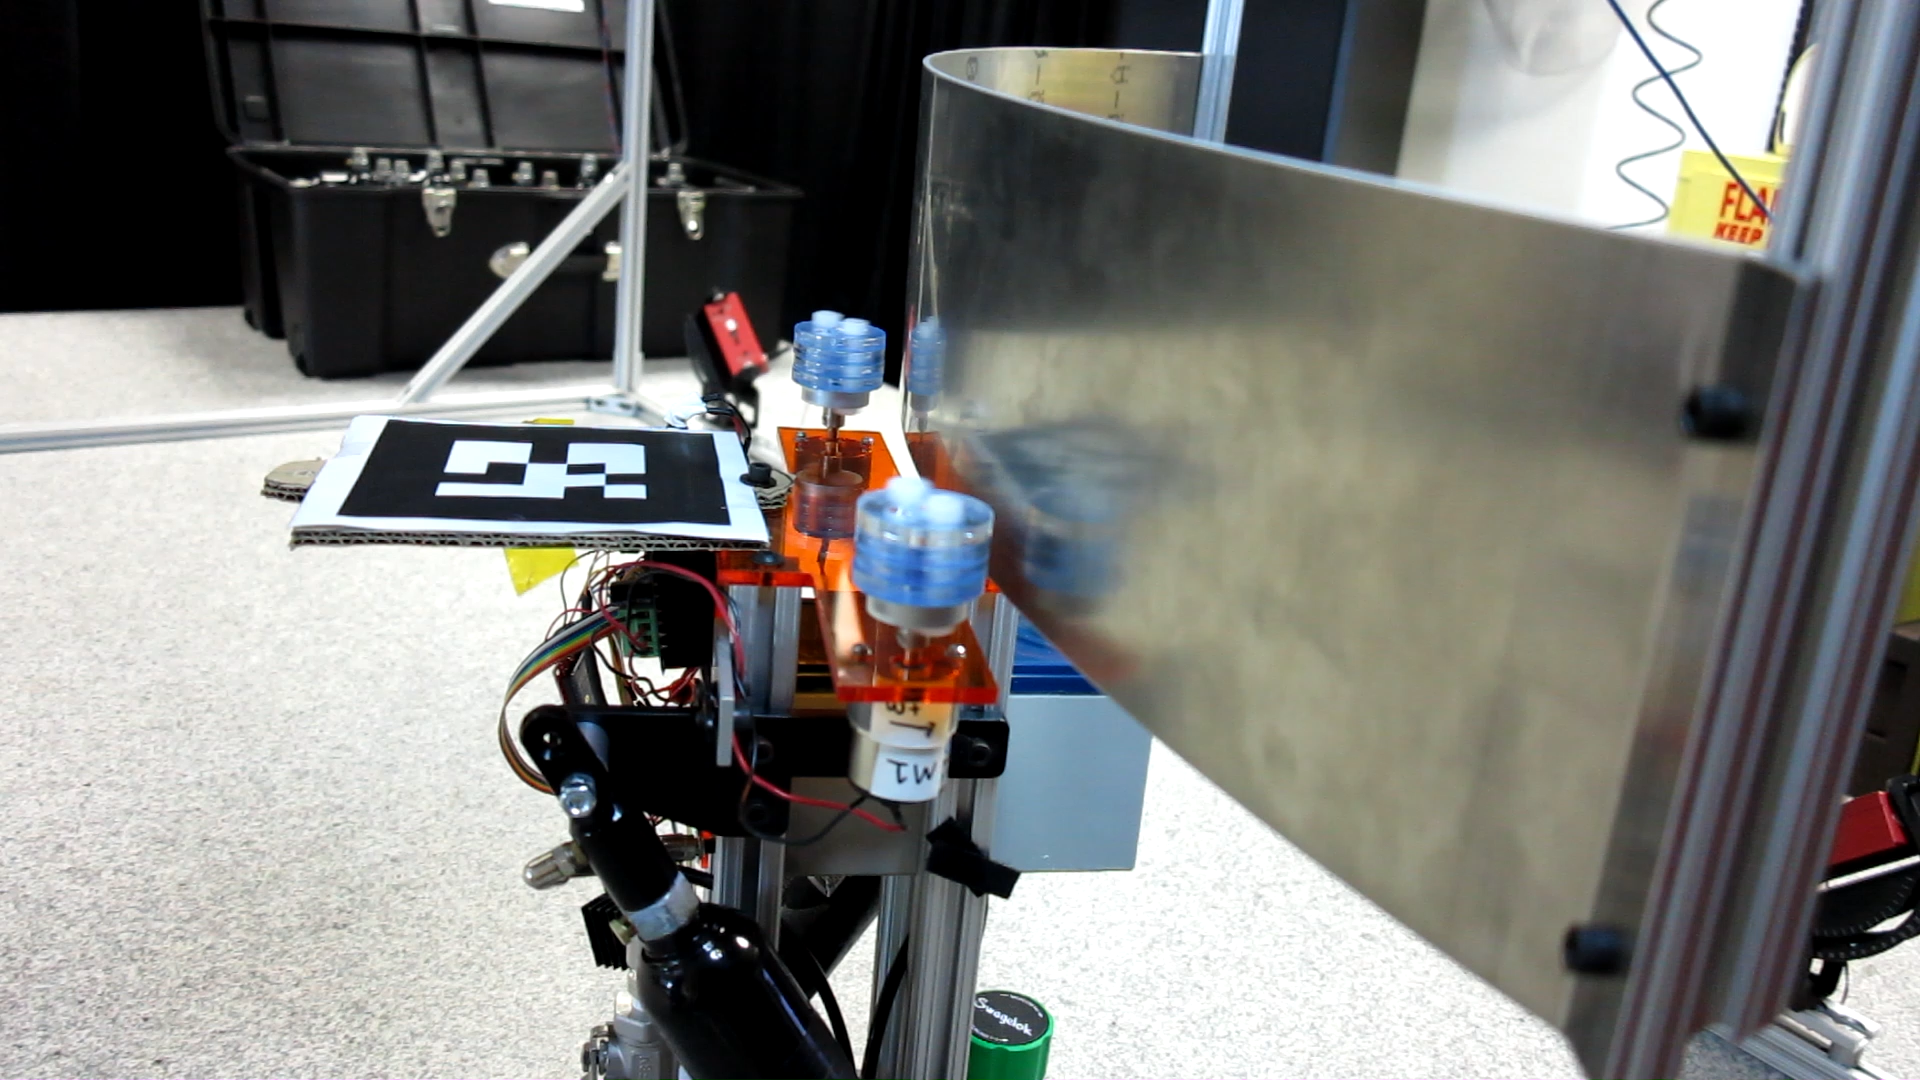
\includegraphics[width = 1.0\linewidth]{figures/screenshot.png}
      \caption{An experimental induction coupled inspector moving near a model of the ISS exterior.}
      \label{fig:realpicture}
   \end{figure}
   %

\par Section \ref{sec:model} presents an analytical model to solve for induction coupler forces. Section \ref{sec:movements} describes and simulates the necessary open-loop manoeuvres to move in each dof. Finally, Section \ref{sec:experiments} presents experimental verification of each manoeuvre with a prototype induction coupler system on a low-friction testbed, shown in figure \ref{fig:realpicture}.
%
\section{Actuator Model}
\label{sec:model}
 \begin{figure}[thpb]
      \centering
      %\framebox{\parbox{3in}{We suggest that you use a text box to insert a graphic (which is ideally a 300 dpi TIFF or EPS file, with all fonts embedded) because, in an document, this method is somewhat more stable than directly inserting a picture.}}

      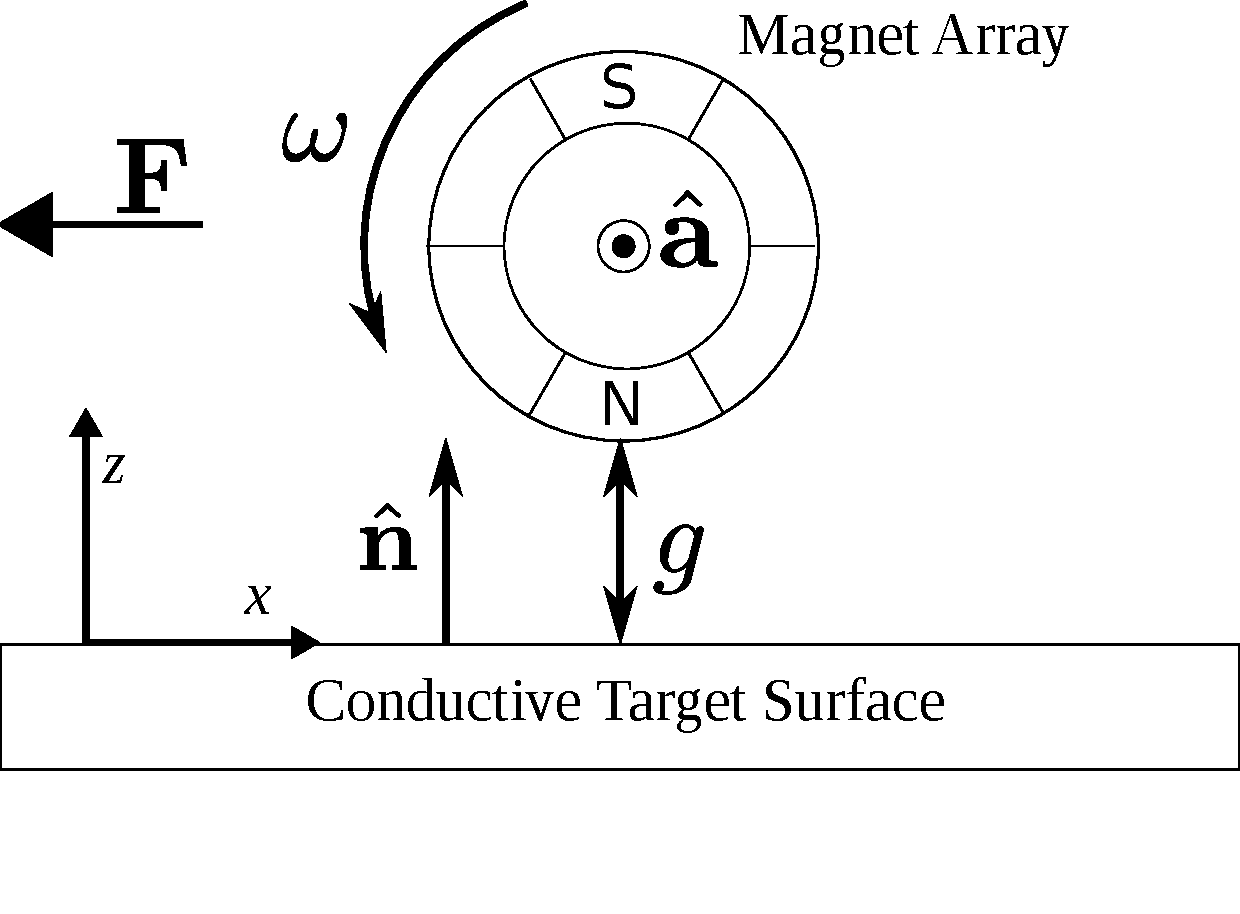
\includegraphics[width = 0.47\textwidth]{figures/spin_mag_diagram.pdf}
      \caption{Diagram of a single induction coupler array}
      \label{fig:single_array}
   \end{figure}
   

Paudel and Bird derived an analytical solution for the force from a single rotating array of permanent magnets near a flat conductor. \cite{Paudel2013} In a reference frame attached to the conductive surface shown in figure \ref{fig:single_array}, the force on the magnet array is

\begin{equation}
\label{eq:Paudel55}
{}^S\textbf{F} = \frac{w}{8\pi\mu_0} \int^{\infty}_{-\infty}\Gamma(\xi,g)|B^s(\xi,g)|^2 d\xi
\end{equation}
%equation explanation.
Where $\Gamma$ is a transmission function associated with the conductive surface and $B$ is the non-time-varying part of the array's magnetic field Fourier transformed with respect to $\hat{x}$.
% 
 $\Gamma$ and $B$ are nonlinear functions of the system state. $\Gamma$ depends on the array's rotation frequency $\omega$, velocity $\textbf{v}$ and distance from the surface $g$. $B$ is a nonlinear function of $g$ as well. Near a curved surface, the assumption of an infinite flat surface is \textit{locally} valid for induction couplers because the operating gap is on the order of centimeters: very small compared to the curvatures of most target surfaces. 
 
\par A geometric generalization of this force is imperative in order to dynamically model the actuation of a 6-DoF orbital inspector. Eddy-current forces act only in opposition to change in magnetic field, so the net force will always act perpendicular to the array's spin axis. Thus, a 3D formulation of the force in any reference frame can be found by tilting the force plane (shown in figure \ref{fig:single_array} along with $\hat{a}$. 

%As the array tilts, $g$ goes from its minimum value when $\hat{\textbf{a}}$ lies in the plane of the surface, to infinity when $\hat{a}$ is perpendicular to the surface. $B$ is proportional to $\frac{1}{g^2}$ so the force will drop to zero when $\hat{\textbf{a}}$ is parallel to the surface. The cross product meets both the conditions on the direction and the magnitude of the force.   

\begin{equation}
\label{eq:arrayForce}
\begin{split}
\textbf{F} =  &F_z(g,\omega,\textbf{v}) \left(\hat{\textbf{a}} \times \hat{\textbf{n}} \right) \\
			 + &F_y(g,\omega,\textbf{v}) \left(\hat{\textbf{a}} \times \hat{\textbf{n}} \right) \times \hat{\textbf{a}}
 \end{split}
 \end{equation}
 
 $F_z$ and $F_y$ are the components of the planar force calculated in equation \ref{eq:Paudel55}
 %
 This statement of eddy-current forces is powerful because it is both analytical and general. The generality enables fast simulations of a 6-DoF inspection vehicle while the analytical nature will enable provable statements about the systems stability.
 %
A full system consists of several arrays to control all six degrees of freedom. The net force and torque on the body then depends on the location and orientation of n arrays in the inspector's frame. Each array rotates around an axis, $\hat{\textbf{a}_n}$, located at $\textbf{d}_n$, shown in figure \ref{fig:planarsetup}. The net control force is 
 
 \begin{equation}
 \label{eq:Fnet }
  \textbf{F}_{net} =  \sum_{i} F_z \left(\hat{\textbf{a}}_i \times \hat{\textbf{n}}_i \right) 
		+ F_y \left(\hat{\textbf{a}}_i \times \hat{\textbf{n}}_i \right) \times \hat{\textbf{a}}_i
 \end{equation}
 
 and the net control torque is
 
 \begin{equation}
 \label{Tnet}
 \boldsymbol{\tau}_{net} =  \sum_{i} \textbf{d}_i \times [F_z \left(\hat{\textbf{a}}_i \times \hat{\textbf{n}}_i \right) 
		+ F_y \left(\hat{\textbf{a}}_i \times \hat{\textbf{n}}_i \right) \times \hat{\textbf{a}}_i]
 \end{equation}

 $\textbf{n}_i$ is the vector to the surface segment closest to array $i$.   
 
\par The following sections use this model to demonstrate how a robotic inspector can use induction couplers to generate forces and torques in all six rigid body degrees of freedom.

%
%The force on a conductive surface from a cyclic magnetic source %\begin{equation}
%\label{eq:sourcefield}
%B = B^s e^{i\omega t}
%\end{equation}
%is given by 
%\begin{equation}
%\label{eq:ForceInt}
%F^{ss} = \frac{w}{8\pi\mu_0}\int_{-\infty}^{\infty}\Gamma\left(\xi \right )\|B^s\left(\xi\right)\|d\xi
%\end{equation}
%here $B^s(\xi)$ is the Fourier transform of the static component of an oscillating source field  and $\Gamma(\xi)$ is a transmission function given in \cite{Paudel2013}. 

\section{Movement Primatives}\label{sec:movements}
\subsection{Planar Movement}\label{sec:planar_movement_desc}
While moving in the plane parallel to the target surface, induction couplers act similar to contactless wheels - they generate forces parallel to the surface that increase with their speed. Thus, a fixed arrangement needs at least two couplers to move in all three planar degrees of freedom and three couplers to control each degree of freedom independently.    
% 

Unlike wheels, induction couplers do not provide constraint forces perpendicular to their rotation.  
%\matt{The following sentence is confusing. Maybe something about no clutch, or the actuator is an accelertion source?}
They also cannot slip on the surface. So unlike wheels that skid if they accelerate too quickly, induction coupler forces are limited only by the capabilities of their motors. 
%

%\matt{Figures reference here}
 
   \begin{figure}[thpb]
      \centering
      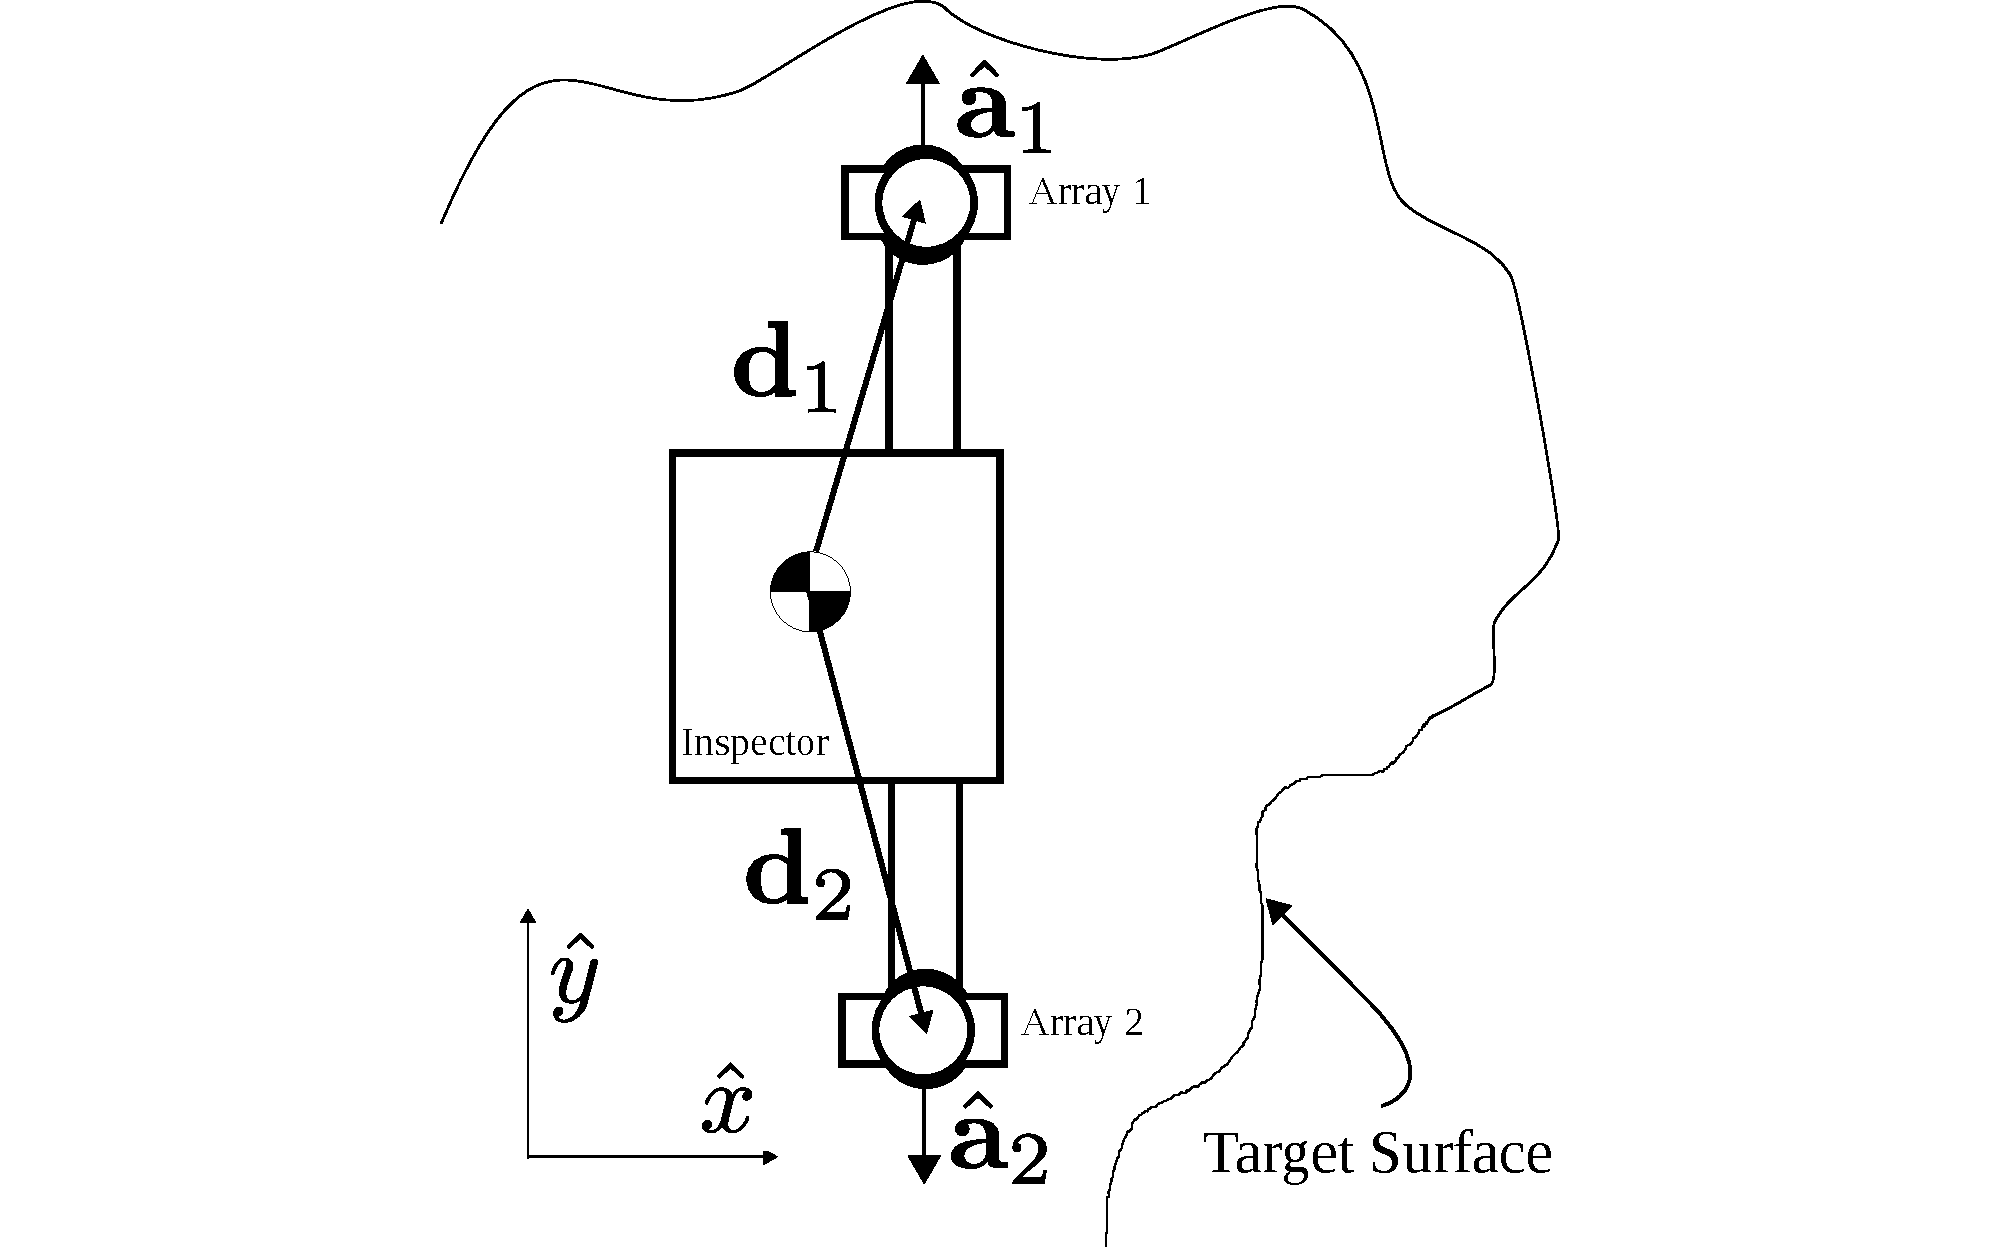
\includegraphics[width = 0.47\textwidth]{figures/surface_locomotion.pdf}
      \caption{Configuration for planar contorl}
      \label{fig:planarsetup}
   \end{figure}

 \par An inspector can translate in the plane by using a pair of induction couplers like differential drive wheels. Figure \ref{fig:planarsetup} shows this mode. Ideally, pure translational motion will involve no net torque. Because there are no kinetic constraints on the couplers the net torque they generate is extremely sensitive to their relative location to the system's center of mass (CoM)\label{def:com}. This sensitivity means that in open loop operation any unaccounted asymmetry between the two induction couplers will lead to unwanted torque. Thus, any induction coupler system will need closed-loop control - the intention of this paper is to demonstrate the raw capabilities of induction couplers and provide the motion primitives that will serve as the foundation for controllers.

%\matt{Simulation of a planar rotation and reversal - need to not have lines on top of eachother - maybe just say curve 1 = curve 2} \ben{done}
      
An inspector also needs to rotate in the plane parallel to the surface. The simplest way for induction couplers to produce pure rotation is to act similarly to differential drive wheels. Two couplers with axes parallel to the surface spin in opposite directions.

 

%Define 'planar torque as torque perpendicular to the plane

%TODO Pseudocode for algorithm 
\subsection{Out-of-Plane Movement}\label{sec:oop_movement_desc}

It is more complicated for induction couplers to produce forces and torques that control movement out of the plane parallel to the target surface because the forces from a single induction coupler are limited in their direction. 

  \begin{figure}[thpb]
      \centering
      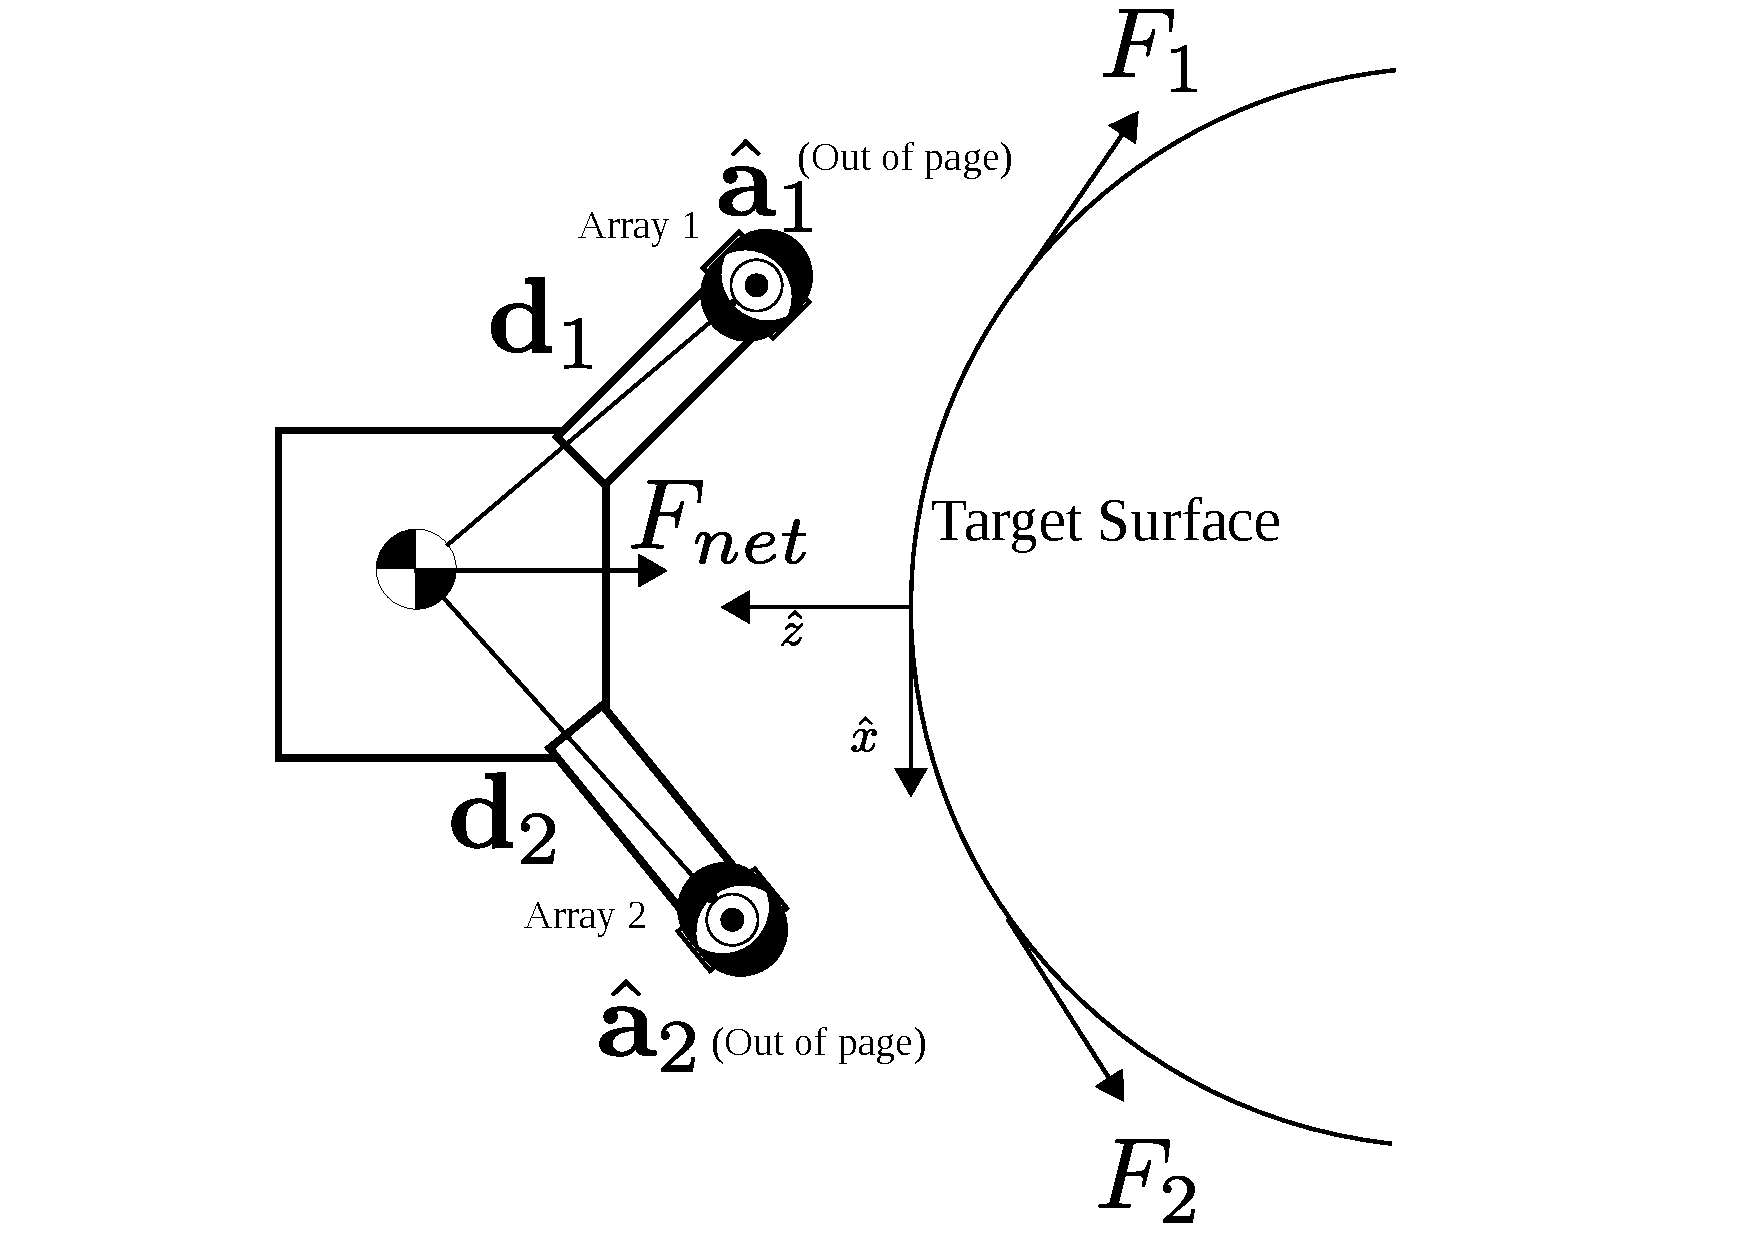
\includegraphics[width = 0.47\textwidth]{figures/curve_locomotion.pdf}
      \caption{Configuration for out-of-plane control}
      \label{fig:oopsetup}
   \end{figure}
   
%Translation
\par The forces generated by spinning arrays are locally almost completely tangential to the surface. For large $\omega$, the ratio of the normal to tangential components of the force increases slightly and can be used to repel away from the surface. However, these forces are small and only act in the $+\hat{\textbf{z}}$ direction, giving no control in $-\hat{\textbf{z}}$. By strategically summing forces across several arrays near different locations on a \textit{non-flat} surface, the inspector can generate larger net forces in both $+\hat{\textbf{z}}$ and $-\hat{\textbf{z}}$. 

\par Rotating two arrays oriented along the $\hat{\textbf{y}}$ with opposing $\omega$ will create local forces who's $\hat{\textbf{x}}$ components will cancel and who's $\hat{\textbf{z}}$ components will sum to pull the inspector towards the surface or push it away. This strategy is illustrated in figure \ref{fig:oopsetup}.     
%Rotation  
\par Using locally tangential forces, the inspector can control rotation about the $\hat{\textbf{y}}$ axis by giving each array the same input speed $\omega$. With only two arrays, the torque is coupled with a force - a third array would make the force and torque independent. 
   


\section{Simulated Demonstration}\label{sec:simulations}

In this section, simulations demonstrate movement with each strategy - planar translation, planar rotation, out-of-plane translation, and out-of-plane rotation in an ideal situation. In each case, the simulation constrains the inspector to the plane of interest to demonstrate open-loop motion primatives - in practice, a closed loop controller is absolutely essential to account for motion out of the plane. The inspector was modelled as a small satellite using two motors with two magnets each as induction couplers. We chose maximum and minimum motor speed inputs to match those used in the experimental demonstrations (section \ref{sec:experiments}.)     

\begin{table}[h]
\caption{Simulation Parameters}
\label{table: sim_params}
\begin{center}
\begin{tabular}{| c | c | c |}
\hline
Description & value & units \\
\hline \hline
Power Consumed at Maximum Input, $P$ & 4 & W \\ \hline

Mass $m$ & 10.2 & kg \\ \hline

Inertia $\textbf{J}$ & $1.02 \mathbb{I}$ & kgm$^2$ \\ \hline

Gap in Planar Movement $g$ & 1 & cm \\ \hline

Conductivity, $\sigma$ & 2.5 $\times 10^7$ & Sm$^{-1}$ \\ \hline

Curvature of non-flat target, $\kappa$  & 0.14 & m$^{-1}$\\

\hline
\end{tabular}
\end{center}
\end{table}

\subsection{Planar Movement}\label{sec:planar_movement_sim}
To demonstrate planar movement, the target is a flat plate in the x-y plane, just like figure \ref{fig:planarsetup}. 
  
     \begin{figure}[thpb]
      	\centering
  		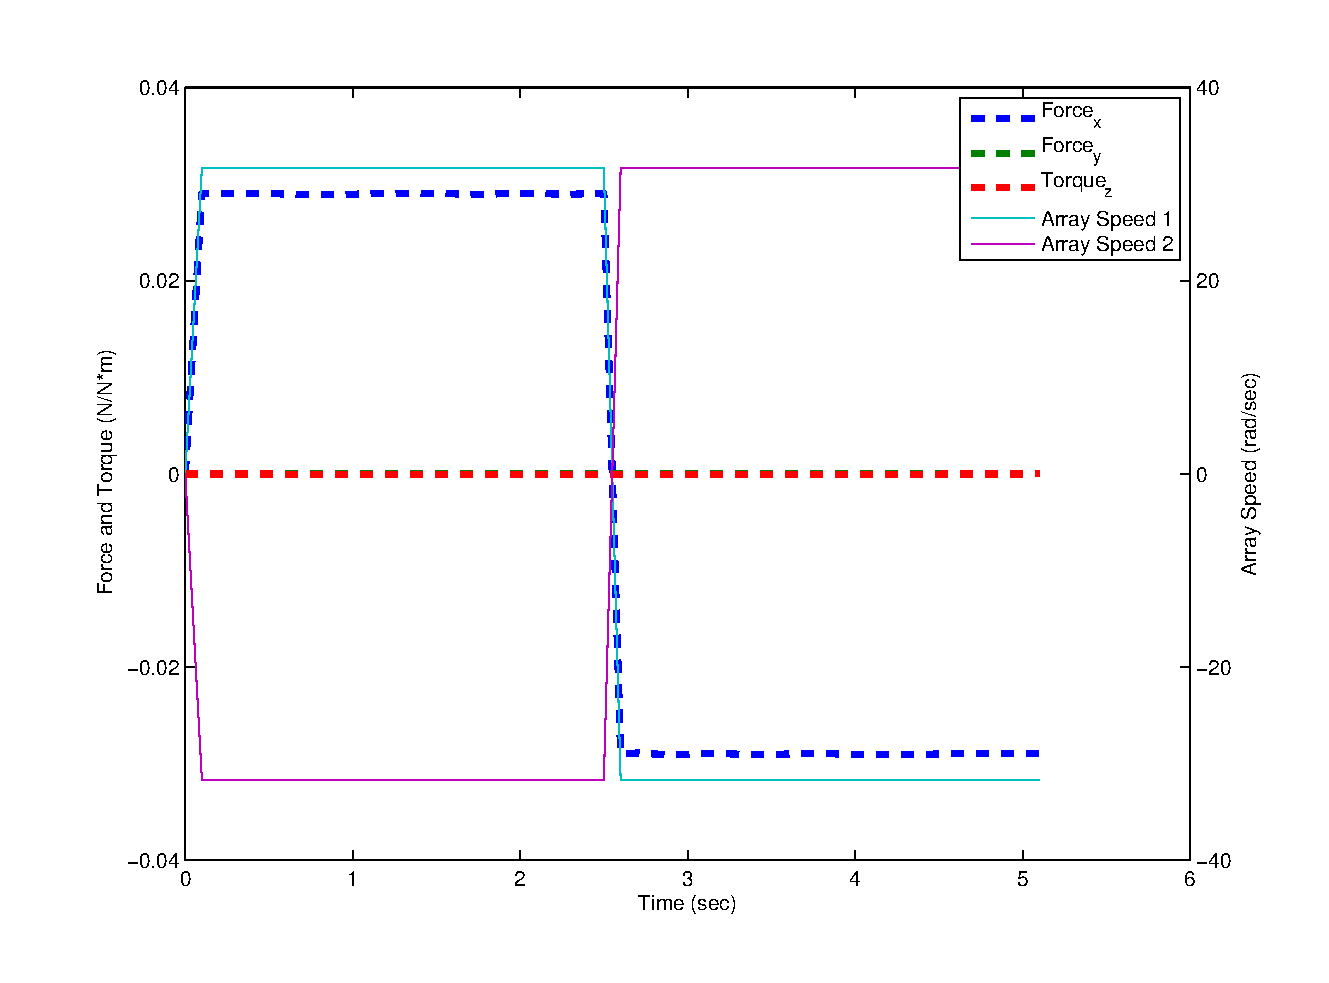
\includegraphics[width = 0.47\textwidth]{figures/planar_translation_sim.eps}
      		\caption{Simulation of planar translation and reversal}
      		\label{fig:planar_translation_sim}
   \end{figure}
   
In figure \ref{fig:planar_translation_sim} the inspector drives itself forward and backwards with 30 mN of force by spinning both arrays forward. Note that $\hat{\textbf{a}}_1 = -\hat{\textbf{a}}_2$.  

     \begin{figure}[thpb]
      \centering
      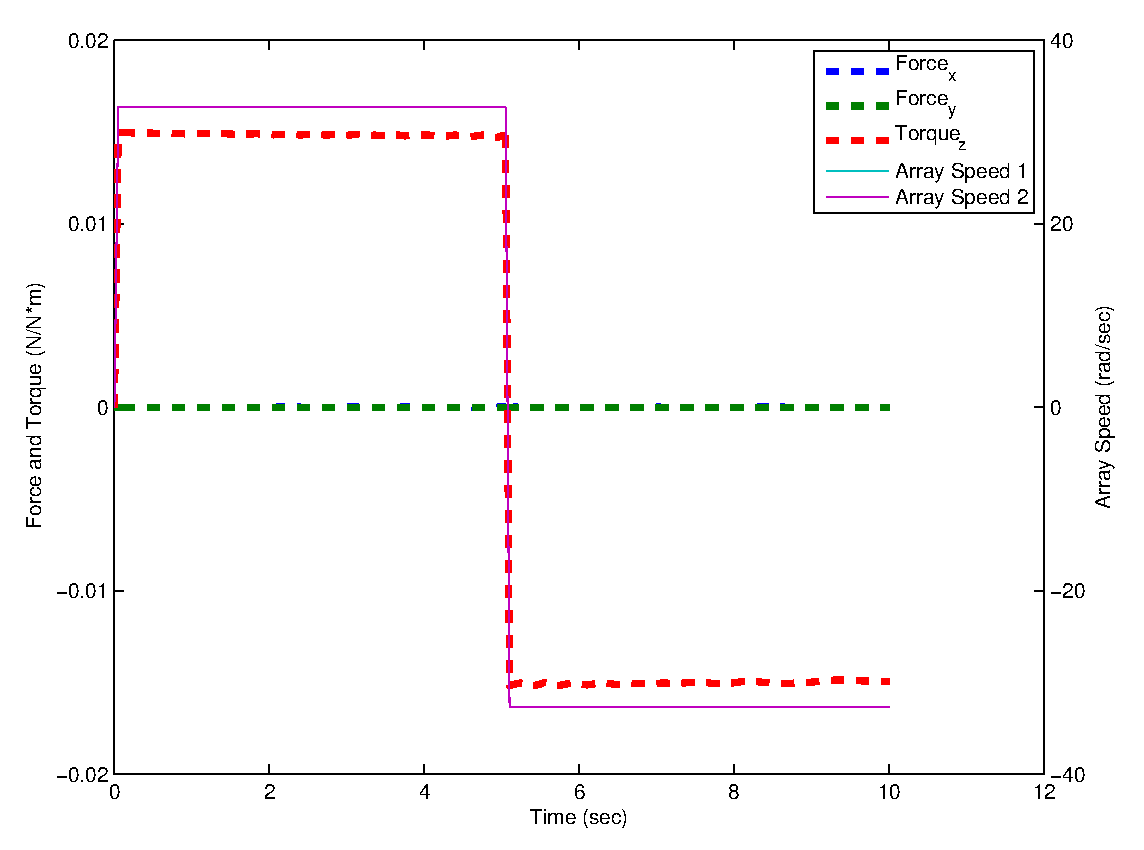
\includegraphics[width = 0.47\textwidth]{figures/planar_rotations.eps}
      \caption{Simulation of planar rotation and reversal. Note: the control speed is the same for both arrays.}
      \label{fig:planar_rotation_sim}
   \end{figure}
   
In figure \ref{fig:planar_rotation_sim} the inspector rotates itself with 15 mN$\cdot$m of torque by counter-spinning each array. 

\subsection{Out-of-Plane Movement}\label{sec:oop_movement_sim}
To demonstrate planar movement the target is a curved in the x-z plane, just like figure \ref{fig:oopsetup} 
The simulation of $\hat{\textbf{z}}$ motion used a target surface with the same curvature as an ISS module. It demonstrates the ability of an induction-coupled inspector to pull itself towards the surface and then push itself away again before colliding. 
     \begin{figure}[thpb]
      \centering
      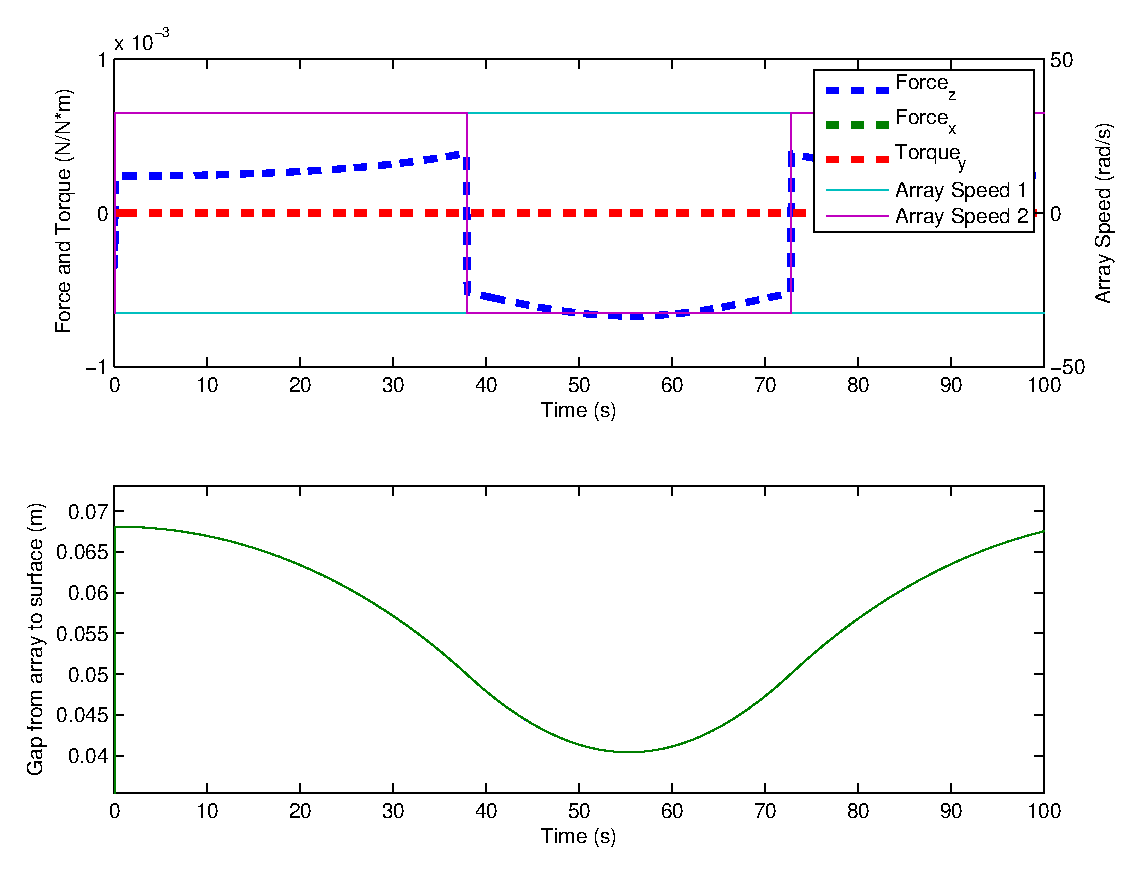
\includegraphics[width = 0.47\textwidth]{figures/curve_translations.eps}
      \caption{Simulation of out-of-plane translation - first pulling on, and then pushing away from the target surface}
      \label{fig:oop_translation_sim}
   \end{figure}
   
   \begin{figure}[thpb]
      \centering
      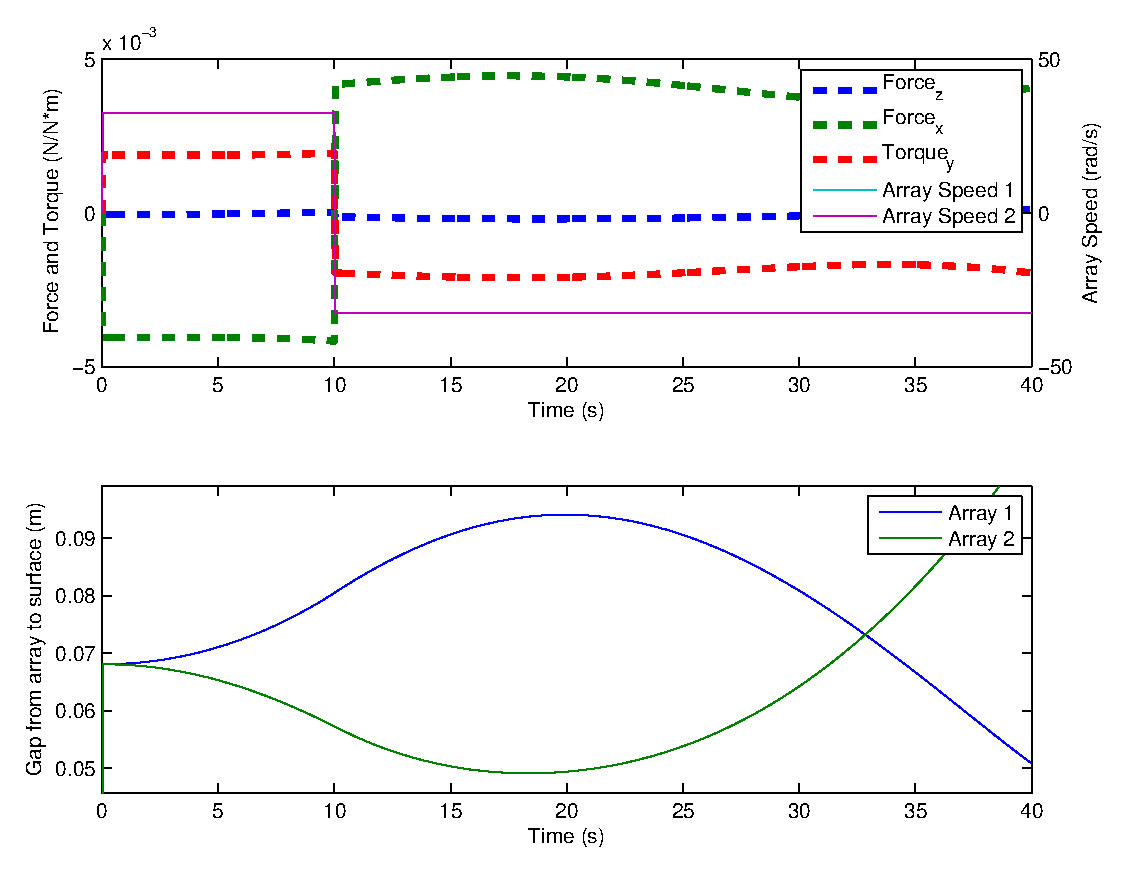
\includegraphics[width = 0.47\textwidth]{figures/curve_rotations.eps}
      \caption{Simulation of out-of-plane rotation - rotating in the +Y and then -Y direction}
      \label{fig:oop_rotation_sim}
   \end{figure}

\section{Experimental Demonstration}\label{sec:experiments}
This section presents an experimental demonstration of each strategy - planar translation, planar rotation, out-of-plane translation, and out-of-plane rotation in an ideal situation. We constructed two prototype inspection vehicles, each with two spinning magnet arrays - one to demonstrate planar movement, one-to-demonstrate out of plane movement. 

\par \textbf{Considerations}: The arrays could not be placed symmetrically about the center of mass due to the constraints of the test platform. Similarly, the tracking points could not be located at the center of mass because the target surface would occult it from the tracking system. These constraints mean that the experiments only serve as a demonstration of the motion primitives for now, rather than a full model validation. 

\subsection{Planar Movement}\label{sec:planar_movement_exp}
   
   \begin{figure}[thpb]
      \centering
      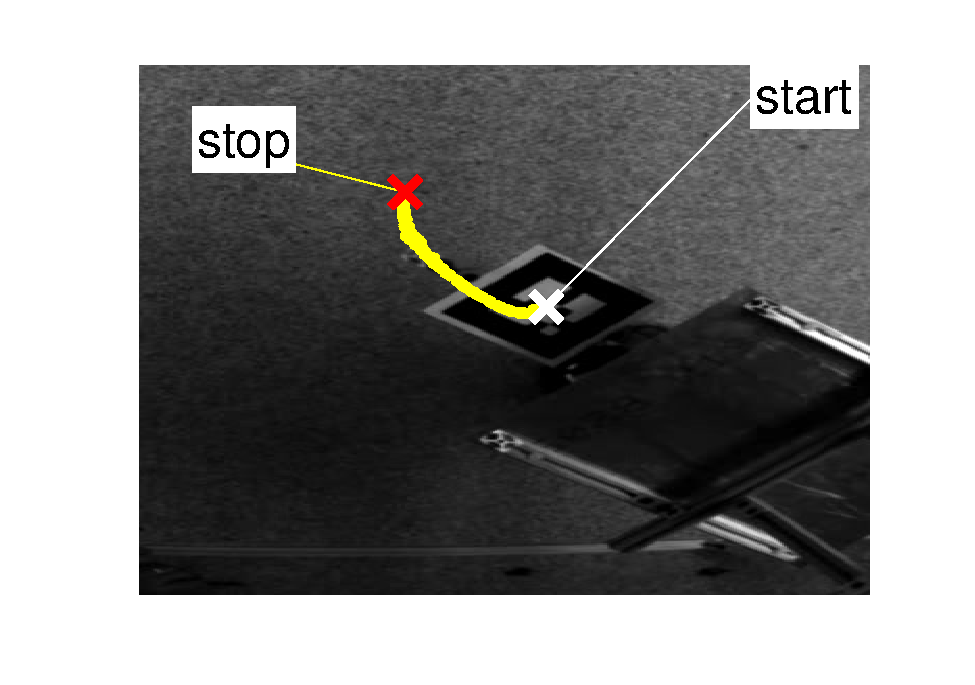
\includegraphics[width = 0.47\textwidth]{figures/planar_translation.eps}
      \caption{Trajectory during open-loop orientation and planar translation}
      \label{fig:planar_translation_exp_trajectory}
   \end{figure}
   
   Figure \ref{fig:planar_translation_exp_trajectory} shows the trajectory of the inspector during planar translation. The inspector spins both arrays forward to translate forward. Unfortunately, the majority of the inspector is obscured because it needs to remain under the plate to push off of it. 
   

      \begin{figure}[thpb]
      \centering
      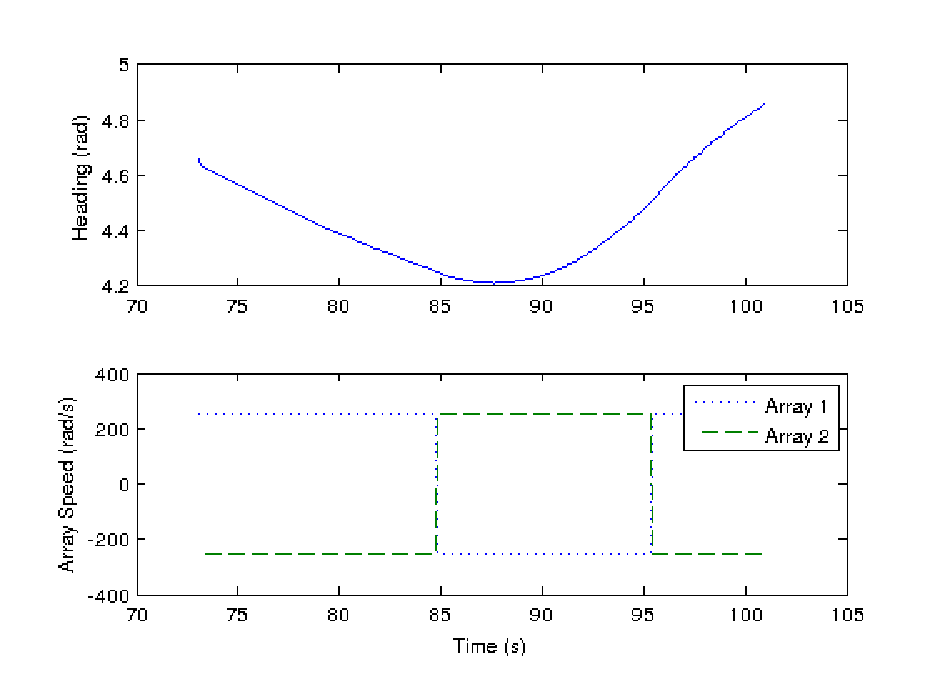
\includegraphics[width = 0.47\textwidth]{figures/planar_rotation.eps}
      \caption{Heading and control input during open-loop planar rotation}
      \label{fig:planar_rotation_exp}
   \end{figure}
   
  \par Figure \ref{fig:planar_rotation_exp} shows a maneuver in which the inspector torqued itself around the $-\textbf{z}$ axis and then stoped and reversed its motion by generating torque around $+\textbf{z}$.  Note that $\hat{\textbf{a}}_1 =  \hat{\textbf{a}}_2$, the opposite of the simulations.

     \subsection{Out-of-Plane Movement}\label{sec:oop_movement_exp}
     
     The plate used to demonstrate out-of-plane movement has a curvature designed to match the harmony module of the ISS. The inspector has two arrays, both with axes pointing in the $-\textbf{y}$ direction, out of the page.  
         \begin{figure}[thpb]
      \centering
      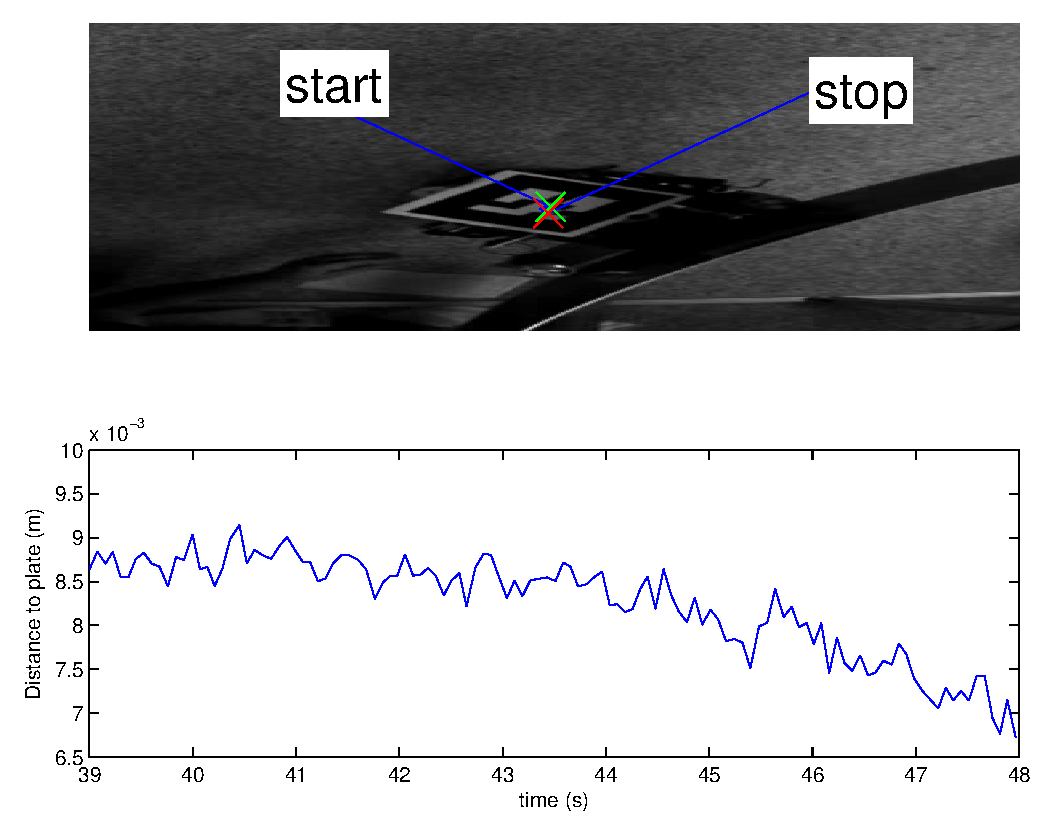
\includegraphics[width = 0.47\textwidth]{figures/oop_translation.eps}
      \caption{Top: Overhead view of out-of-plane demonstration Bottom: distance to plate during out-of-plane translation}
      \label{fig:oop_translation_exp}
   \end{figure}
   
   \par Figure \ref{fig:oop_translation_exp} shows the results from the inspector pulling itself towards the surface. Unfortunately, the distance it could travel before colliding with the plate was tiny - a clear reason for closed-loop control. The bottom half of the figure shows that the inspector does in fact accelerate towards the surface - the gap decreases with an increasing rate. 
  
      
         \begin{figure}[thpb]
      \centering
      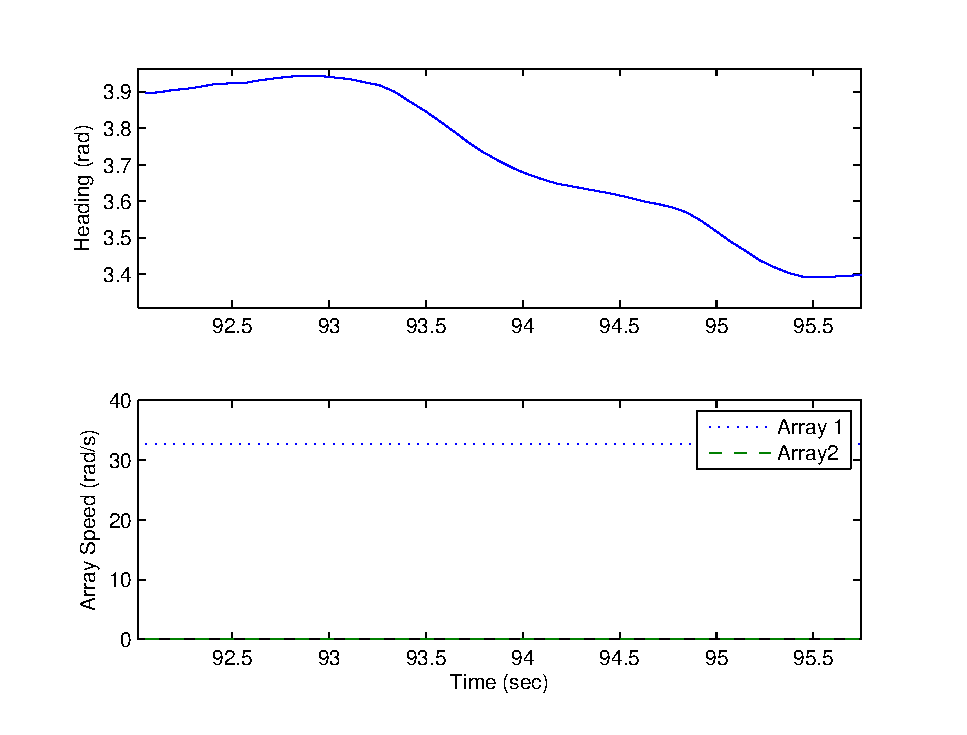
\includegraphics[width = 0.47\textwidth]{figures/oop_rotation.eps}
      \caption{Heading during out-of-plane rotation}
      \label{fig:oop_rotation_exp}
   \end{figure}
   
   \par Figure \ref{fig:oop_rotation_exp} shows the heading of the inspector as it rotates itself out of the plane about the $\hat{\textbf{y}}$ axis.



\section{Conclusion}
A robotic on-orbit service vehicle can use induction couplers can produce locomotive forces in all six rigid body degrees of freedom near a conductive surface. Rotating permanent-magnet arrays generate forces perpendicular to both their axes of rotation and the conductive surface. Current-oscillating electromagnets generate forces directly away from the surface. A pair of rotating arrays can produce $\hat{x}$ and $\hat{y}$ forces in the plane of the traversal surface. These two arrays can also produce torques in the $\hat{z}$ direction. This pair of arrays can take advantage of the surface geometry to generate forces in the $\hat{z}$ direction by generating shear forces along a non-flat surface whose $\hat{x}$ and $\hat{y}$ components cancel but whose $\hat{s}$ components add. A single electromagnet generates force in the $+\hat{z}$ direction. The force from the electromagnet can also generate torques based on its relative location to the system's center of mass. These maneuvers are demonstrated in simulations and verified on a low-friction testbed.  

%An autonomous space vehicle can use these forces to crawl over the conductive surface of a target spacecraft without propellant or the risk associated with physical grappling. Rotating arrays of magnets produce planar forces and torques. These rotating arrays can also produce forces perpendicular to the surface by taking advantage of surface features such as curvature or edges. Electromagnets can produce force directly away from any surface and by coupling these forces, produce torques parallel to that surface. Dynamic simulations demonstrate each degree-of-freedom using an analytical force model and hardware demonstrations on a low-friction testbed verify the results. 
%TODO future work - trajectory optimization, end effector design, kinematic simulation
Future work will focus on two areas - adaptive controllers and movement planning. A robotic inspector will need adaptive controllers to account for induction coupler's strong dependence on poorly known parameters of the environment.  The inspector will also need to plan movements carefully because its ability to exert control with an induction coupler is based on both its state and the local geometry.      





   


\addtolength{\textheight}{-12cm}   % This command serves to balance the column lengths
                                  % on the last page of the document manually. It shortens
                                  % the textheight of the last page by a suitable amount.
                                  % This command does not take effect until the next page
                                  % so it should come on the page before the last. Make
                                  % sure that you do not shorten the textheight too much.

%%%%%%%%%%%%%%%%%%%%%%%%%%%%%%%%%%%%%%%%%%%%%%%%%%%%%%%%%%%%%%%%%%%%%%%%%%%%%%%%



%%%%%%%%%%%%%%%%%%%%%%%%%%%%%%%%%%%%%%%%%%%%%%%%%%%%%%%%%%%%%%%%%%%%%%%%%%%%%%%%



%%%%%%%%%%%%%%%%%%%%%%%%%%%%%%%%%%%%%%%%%%%%%%%%%%%%%%%%%%%%%%%%%%%%%%%%%%%%%%%%

\section*{ACKNOWLEDGMENT}
This work was supported by a NSTRF Grant.



%%%%%%%%%%%%%%%%%%%%%%%%%%%%%%%%%%%%%%%%%%%%%%%%%%%%%%%%%%%%%%%%%%%%%%%%%%%%%%%%


\bibliographystyle{plain}
\bibliography{biblio.bib}




\end{document}

%TODO SPECIFIC QUESTIONS FOR REVIEWERS
% Are there any terms that are unclear
% Is it clear from the beginning what you are going to be told?
% Does the paper meet hose expectations?